\documentclass[1p]{elsarticle_modified}
%\bibliographystyle{elsarticle-num}

%\usepackage[colorlinks]{hyperref}
%\usepackage{abbrmath_seonhwa} %\Abb, \Ascr, \Acal ,\Abf, \Afrak
\usepackage{amsfonts}
\usepackage{amssymb}
\usepackage{amsmath}
\usepackage{amsthm}
\usepackage{scalefnt}
\usepackage{amsbsy}
\usepackage{kotex}
\usepackage{caption}
\usepackage{subfig}
\usepackage{color}
\usepackage{graphicx}
\usepackage{xcolor} %% white, black, red, green, blue, cyan, magenta, yellow
\usepackage{float}
\usepackage{setspace}
\usepackage{hyperref}

\usepackage{tikz}
\usetikzlibrary{arrows}

\usepackage{multirow}
\usepackage{array} % fixed length table
\usepackage{hhline}

%%%%%%%%%%%%%%%%%%%%%
\makeatletter
\renewcommand*\env@matrix[1][\arraystretch]{%
	\edef\arraystretch{#1}%
	\hskip -\arraycolsep
	\let\@ifnextchar\new@ifnextchar
	\array{*\c@MaxMatrixCols c}}
\makeatother %https://tex.stackexchange.com/questions/14071/how-can-i-increase-the-line-spacing-in-a-matrix
%%%%%%%%%%%%%%%

\usepackage[normalem]{ulem}

\newcommand{\msout}[1]{\ifmmode\text{\sout{\ensuremath{#1}}}\else\sout{#1}\fi}
%SOURCE: \msout is \stkout macro in https://tex.stackexchange.com/questions/20609/strikeout-in-math-mode

\newcommand{\cancel}[1]{
	\ifmmode
	{\color{red}\msout{#1}}
	\else
	{\color{red}\sout{#1}}
	\fi
}

\newcommand{\add}[1]{
	{\color{blue}\uwave{#1}}
}

\newcommand{\replace}[2]{
	\ifmmode
	{\color{red}\msout{#1}}{\color{blue}\uwave{#2}}
	\else
	{\color{red}\sout{#1}}{\color{blue}\uwave{#2}}
	\fi
}

\newcommand{\Sol}{\mathcal{S}} %segment
\newcommand{\D}{D} %diagram
\newcommand{\A}{\mathcal{A}} %arc


%%%%%%%%%%%%%%%%%%%%%%%%%%%%%5 test

\def\sl{\operatorname{\textup{SL}}(2,\Cbb)}
\def\psl{\operatorname{\textup{PSL}}(2,\Cbb)}
\def\quan{\mkern 1mu \triangleright \mkern 1mu}

\theoremstyle{definition}
\newtheorem{thm}{Theorem}[section]
\newtheorem{prop}[thm]{Proposition}
\newtheorem{lem}[thm]{Lemma}
\newtheorem{ques}[thm]{Question}
\newtheorem{cor}[thm]{Corollary}
\newtheorem{defn}[thm]{Definition}
\newtheorem{exam}[thm]{Example}
\newtheorem{rmk}[thm]{Remark}
\newtheorem{alg}[thm]{Algorithm}

\newcommand{\I}{\sqrt{-1}}
\begin{document}

%\begin{frontmatter}
%
%\title{Boundary parabolic representations of knots up to 8 crossings}
%
%%% Group authors per affiliation:
%\author{Yunhi Cho} 
%\address{Department of Mathematics, University of Seoul, Seoul, Korea}
%\ead{yhcho@uos.ac.kr}
%
%
%\author{Seonhwa Kim} %\fnref{s_kim}}
%\address{Center for Geometry and Physics, Institute for Basic Science, Pohang, 37673, Korea}
%\ead{ryeona17@ibs.re.kr}
%
%\author{Hyuk Kim}
%\address{Department of Mathematical Sciences, Seoul National University, Seoul 08826, Korea}
%\ead{hyukkim@snu.ac.kr}
%
%\author{Seokbeom Yoon}
%\address{Department of Mathematical Sciences, Seoul National University, Seoul, 08826,  Korea}
%\ead{sbyoon15@snu.ac.kr}
%
%\begin{abstract}
%We find all boundary parabolic representation of knots up to 8 crossings.
%
%\end{abstract}
%\begin{keyword}
%    \MSC[2010] 57M25 
%\end{keyword}
%
%\end{frontmatter}

%\linenumbers
%\tableofcontents
%
\newcommand\colored[1]{\textcolor{white}{\rule[-0.35ex]{0.8em}{1.4ex}}\kern-0.8em\color{red} #1}%
%\newcommand\colored[1]{\textcolor{white}{ #1}\kern-2.17ex	\textcolor{white}{ #1}\kern-1.81ex	\textcolor{white}{ #1}\kern-2.15ex\color{red}#1	}

{\Large $\underline{12a_{1017}~(K12a_{1017})}$}

\setlength{\tabcolsep}{10pt}
\renewcommand{\arraystretch}{1.6}
\vspace{1cm}\begin{tabular}{m{100pt}>{\centering\arraybackslash}m{274pt}}
\multirow{5}{120pt}{
	\centering
	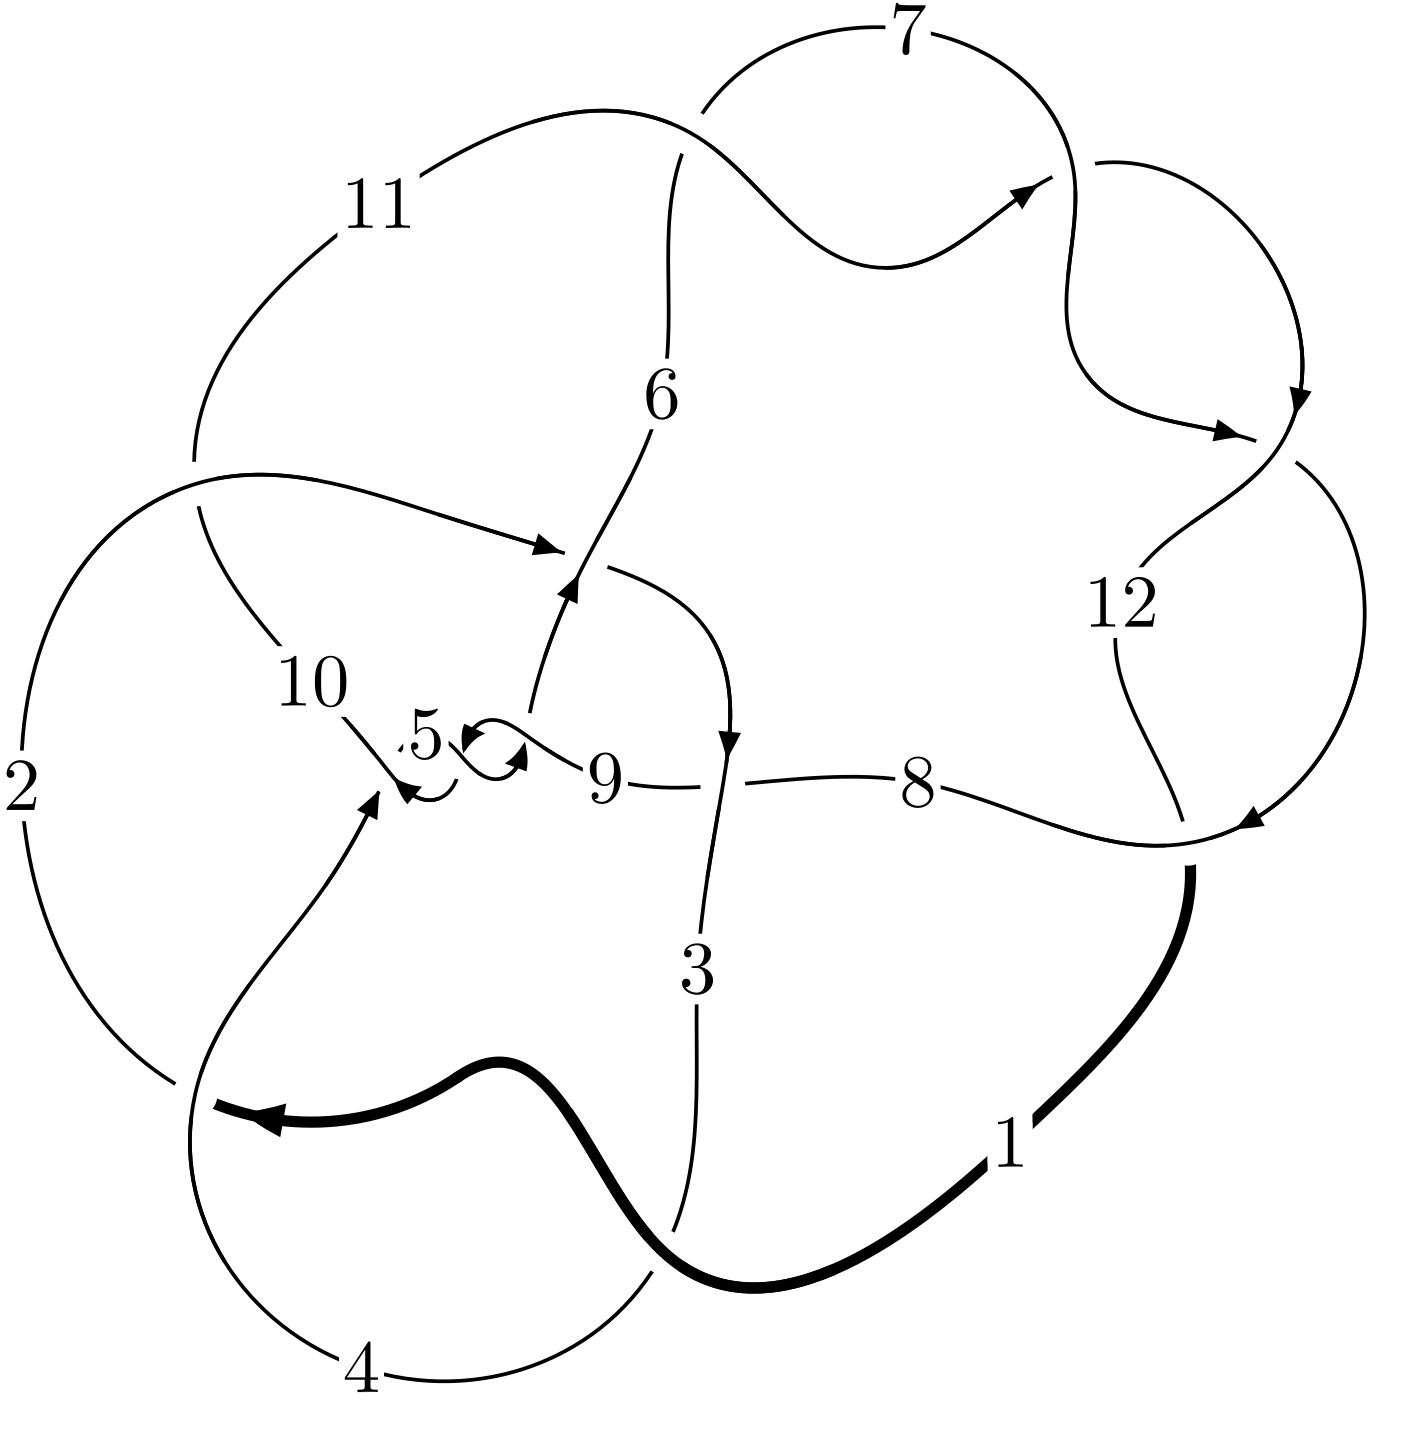
\includegraphics[width=112pt]{../../../GIT/diagram.site/Diagrams/png/1818_12a_1017.png}\\
\ \ \ A knot diagram\footnotemark}&
\allowdisplaybreaks
\textbf{Linearized knot diagam} \\
\cline{2-2}
 &
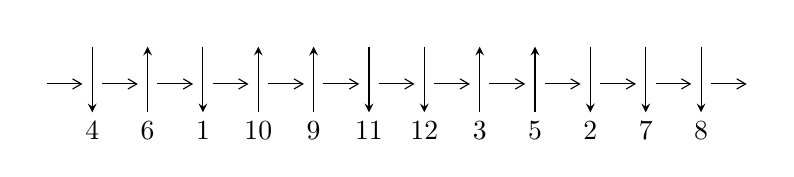
\begin{tikzpicture}[x=20pt, y=17pt]
	% nodes
	\node (C0) at (0, 0) {};
	\node (C1) at (1, 0) {};
	\node (C1U) at (1, +1) {};
	\node (C1D) at (1, -1) {4};

	\node (C2) at (2, 0) {};
	\node (C2U) at (2, +1) {};
	\node (C2D) at (2, -1) {6};

	\node (C3) at (3, 0) {};
	\node (C3U) at (3, +1) {};
	\node (C3D) at (3, -1) {1};

	\node (C4) at (4, 0) {};
	\node (C4U) at (4, +1) {};
	\node (C4D) at (4, -1) {10};

	\node (C5) at (5, 0) {};
	\node (C5U) at (5, +1) {};
	\node (C5D) at (5, -1) {9};

	\node (C6) at (6, 0) {};
	\node (C6U) at (6, +1) {};
	\node (C6D) at (6, -1) {11};

	\node (C7) at (7, 0) {};
	\node (C7U) at (7, +1) {};
	\node (C7D) at (7, -1) {12};

	\node (C8) at (8, 0) {};
	\node (C8U) at (8, +1) {};
	\node (C8D) at (8, -1) {3};

	\node (C9) at (9, 0) {};
	\node (C9U) at (9, +1) {};
	\node (C9D) at (9, -1) {5};

	\node (C10) at (10, 0) {};
	\node (C10U) at (10, +1) {};
	\node (C10D) at (10, -1) {2};

	\node (C11) at (11, 0) {};
	\node (C11U) at (11, +1) {};
	\node (C11D) at (11, -1) {7};

	\node (C12) at (12, 0) {};
	\node (C12U) at (12, +1) {};
	\node (C12D) at (12, -1) {8};
	\node (C13) at (13, 0) {};

	% arrows
	\draw[->,>={angle 60}]
	(C0) edge (C1) (C1) edge (C2) (C2) edge (C3) (C3) edge (C4) (C4) edge (C5) (C5) edge (C6) (C6) edge (C7) (C7) edge (C8) (C8) edge (C9) (C9) edge (C10) (C10) edge (C11) (C11) edge (C12) (C12) edge (C13) ;	\draw[->,>=stealth]
	(C1U) edge (C1D) (C2D) edge (C2U) (C3U) edge (C3D) (C4D) edge (C4U) (C5D) edge (C5U) (C6U) edge (C6D) (C7U) edge (C7D) (C8D) edge (C8U) (C9D) edge (C9U) (C10U) edge (C10D) (C11U) edge (C11D) (C12U) edge (C12D) ;
	\end{tikzpicture} \\
\hhline{~~} \\& 
\textbf{Solving Sequence} \\ \cline{2-2} 
 &
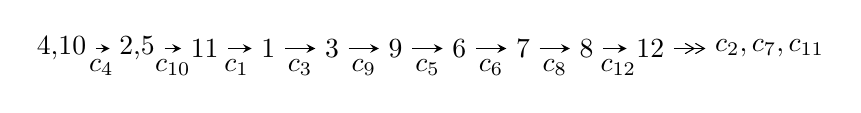
\begin{tikzpicture}[x=23pt, y=7pt]
	% node
	\node (A0) at (-1/8, 0) {4,10};
	\node (A1) at (17/16, 0) {2,5};
	\node (A2) at (17/8, 0) {11};
	\node (A3) at (25/8, 0) {1};
	\node (A4) at (33/8, 0) {3};
	\node (A5) at (41/8, 0) {9};
	\node (A6) at (49/8, 0) {6};
	\node (A7) at (57/8, 0) {7};
	\node (A8) at (65/8, 0) {8};
	\node (A9) at (73/8, 0) {12};
	\node (C1) at (1/2, -1) {$c_{4}$};
	\node (C2) at (13/8, -1) {$c_{10}$};
	\node (C3) at (21/8, -1) {$c_{1}$};
	\node (C4) at (29/8, -1) {$c_{3}$};
	\node (C5) at (37/8, -1) {$c_{9}$};
	\node (C6) at (45/8, -1) {$c_{5}$};
	\node (C7) at (53/8, -1) {$c_{6}$};
	\node (C8) at (61/8, -1) {$c_{8}$};
	\node (C9) at (69/8, -1) {$c_{12}$};
	\node (A10) at (11, 0) {$c_{2},c_{7},c_{11}$};

	% edge
	\draw[->,>=stealth]	
	(A0) edge (A1) (A1) edge (A2) (A2) edge (A3) (A3) edge (A4) (A4) edge (A5) (A5) edge (A6) (A6) edge (A7) (A7) edge (A8) (A8) edge (A9) ;
	\draw[->>,>={angle 60}]	
	(A9) edge (A10);
\end{tikzpicture} \\ 

\end{tabular} \\

\footnotetext{
The image of knot diagram is generated by the software ``\textbf{Draw programme}" developed by Andrew Bartholomew(\url{http://www.layer8.co.uk/maths/draw/index.htm\#Running-draw}), where we modified some parts for our purpose(\url{https://github.com/CATsTAILs/LinksPainter}).
}\phantom \\ \newline 
\centering \textbf{Ideals for irreducible components\footnotemark of $X_{\text{par}}$} 
 
\begin{align*}
I^u_{1}&=\langle 
-2.60368\times10^{56} u^{58}+4.19299\times10^{56} u^{57}+\cdots+1.57047\times10^{57} b+1.44031\times10^{57},\\
\phantom{I^u_{1}}&\phantom{= \langle  }-1.44721\times10^{58} u^{58}+2.32648\times10^{58} u^{57}+\cdots+1.72751\times10^{58} a-2.18987\times10^{58},\;u^{59}-2 u^{58}+\cdots+2 u-1\rangle \\
I^u_{2}&=\langle 
b+1,\;-6 u^4- u^3-4 u^2+11 a-6 u-2,\;u^5- u^4+2 u^3- u^2+u-1\rangle \\
\\
\end{align*}
\raggedright * 2 irreducible components of $\dim_{\mathbb{C}}=0$, with total 64 representations.\\
\footnotetext{All coefficients of polynomials are rational numbers. But the coefficients are sometimes approximated in decimal forms when there is not enough margin.}
\newpage
\renewcommand{\arraystretch}{1}
\centering \section*{I. $I^u_{1}= \langle -2.60\times10^{56} u^{58}+4.19\times10^{56} u^{57}+\cdots+1.57\times10^{57} b+1.44\times10^{57},\;-1.45\times10^{58} u^{58}+2.33\times10^{58} u^{57}+\cdots+1.73\times10^{58} a-2.19\times10^{58},\;u^{59}-2 u^{58}+\cdots+2 u-1 \rangle$}
\flushleft \textbf{(i) Arc colorings}\\
\begin{tabular}{m{7pt} m{180pt} m{7pt} m{180pt} }
\flushright $a_{4}=$&$\begin{pmatrix}1\\0\end{pmatrix}$ \\
\flushright $a_{10}=$&$\begin{pmatrix}0\\u\end{pmatrix}$ \\
\flushright $a_{2}=$&$\begin{pmatrix}0.837744 u^{58}-1.34673 u^{57}+\cdots+9.36260 u+1.26764\\0.165790 u^{58}-0.266990 u^{57}+\cdots-0.250227 u-0.917125\end{pmatrix}$ \\
\flushright $a_{5}=$&$\begin{pmatrix}1\\- u^2\end{pmatrix}$ \\
\flushright $a_{11}=$&$\begin{pmatrix}-1.37006 u^{58}+2.70687 u^{57}+\cdots-2.20419 u-7.53648\\0.323082 u^{58}-0.735433 u^{57}+\cdots+0.636173 u+0.712700\end{pmatrix}$ \\
\flushright $a_{1}=$&$\begin{pmatrix}1.00353 u^{58}-1.61372 u^{57}+\cdots+9.11237 u+0.350517\\0.165790 u^{58}-0.266990 u^{57}+\cdots-0.250227 u-0.917125\end{pmatrix}$ \\
\flushright $a_{3}=$&$\begin{pmatrix}0.813781 u^{58}-1.27902 u^{57}+\cdots+9.23409 u+1.12697\\0.101081 u^{58}-0.176699 u^{57}+\cdots-0.139831 u-0.934603\end{pmatrix}$ \\
\flushright $a_{9}=$&$\begin{pmatrix}- u\\u^3+u\end{pmatrix}$ \\
\flushright $a_{6}=$&$\begin{pmatrix}u^2+1\\- u^4-2 u^2\end{pmatrix}$ \\
\flushright $a_{7}=$&$\begin{pmatrix}1.22085 u^{58}-1.69130 u^{57}+\cdots+1.86963 u+5.41585\\-0.341950 u^{58}+0.451068 u^{57}+\cdots+0.714485 u-0.813658\end{pmatrix}$ \\
\flushright $a_{8}=$&$\begin{pmatrix}-1.10578 u^{58}+1.81302 u^{57}+\cdots-8.88249 u-6.38263\\0.522951 u^{58}-1.01970 u^{57}+\cdots-0.297256 u+0.859688\end{pmatrix}$ \\
\flushright $a_{12}=$&$\begin{pmatrix}-0.815570 u^{58}+1.08491 u^{57}+\cdots+7.19499 u-5.10912\\0.485858 u^{58}-0.909085 u^{57}+\cdots-1.03362 u+0.314960\end{pmatrix}$\\&\end{tabular}
\flushleft \textbf{(ii) Obstruction class $= -1$}\\~\\
\flushleft \textbf{(iii) Cusp Shapes $= 2.95860 u^{58}-4.62866 u^{57}+\cdots-1.56836 u+1.88588$}\\~\\
\newpage\renewcommand{\arraystretch}{1}
\flushleft \textbf{(iv) u-Polynomials at the component}\newline \\
\begin{tabular}{m{50pt}|m{274pt}}
Crossings & \hspace{64pt}u-Polynomials at each crossing \\
\hline $$\begin{aligned}c_{1},c_{3}\end{aligned}$$&$\begin{aligned}
&u^{59}-6 u^{58}+\cdots-222 u-121
\end{aligned}$\\
\hline $$\begin{aligned}c_{2}\end{aligned}$$&$\begin{aligned}
&u^{59}-5 u^{58}+\cdots-9856 u-3872
\end{aligned}$\\
\hline $$\begin{aligned}c_{4},c_{5},c_{9}\end{aligned}$$&$\begin{aligned}
&u^{59}-2 u^{58}+\cdots+2 u-1
\end{aligned}$\\
\hline $$\begin{aligned}c_{6},c_{7},c_{11}\\c_{12}\end{aligned}$$&$\begin{aligned}
&u^{59}-2 u^{58}+\cdots-2 u-1
\end{aligned}$\\
\hline $$\begin{aligned}c_{8}\end{aligned}$$&$\begin{aligned}
&11(11 u^{59}+7 u^{58}+\cdots-474357 u-87053)
\end{aligned}$\\
\hline $$\begin{aligned}c_{10}\end{aligned}$$&$\begin{aligned}
&11(11 u^{59}+48 u^{58}+\cdots-267960 u+42881)
\end{aligned}$\\
\hline
\end{tabular}\\~\\
\newpage\renewcommand{\arraystretch}{1}
\flushleft \textbf{(v) Riley Polynomials at the component}\newline \\
\begin{tabular}{m{50pt}|m{274pt}}
Crossings & \hspace{64pt}Riley Polynomials at each crossing \\
\hline $$\begin{aligned}c_{1},c_{3}\end{aligned}$$&$\begin{aligned}
&y^{59}-56 y^{58}+\cdots+212150 y-14641
\end{aligned}$\\
\hline $$\begin{aligned}c_{2}\end{aligned}$$&$\begin{aligned}
&y^{59}+33 y^{58}+\cdots-70687232 y-14992384
\end{aligned}$\\
\hline $$\begin{aligned}c_{4},c_{5},c_{9}\end{aligned}$$&$\begin{aligned}
&y^{59}+60 y^{58}+\cdots-8 y-1
\end{aligned}$\\
\hline $$\begin{aligned}c_{6},c_{7},c_{11}\\c_{12}\end{aligned}$$&$\begin{aligned}
&y^{59}-72 y^{58}+\cdots-8 y-1
\end{aligned}$\\
\hline $$\begin{aligned}c_{8}\end{aligned}$$&$\begin{aligned}
&121(121 y^{59}+4725 y^{58}+\cdots+3.57051\times10^{10} y-7.57822\times10^{9})
\end{aligned}$\\
\hline $$\begin{aligned}c_{10}\end{aligned}$$&$\begin{aligned}
&121(121 y^{59}-6660 y^{58}+\cdots+8.46566\times10^{10} y-1.83878\times10^{9})
\end{aligned}$\\
\hline
\end{tabular}\\~\\
\newpage\flushleft \textbf{(vi) Complex Volumes and Cusp Shapes}
$$\begin{array}{c|c|c}  
\text{Solutions to }I^u_{1}& \I (\text{vol} + \sqrt{-1}CS) & \text{Cusp shape}\\
 \hline 
\begin{aligned}
u &= \phantom{-}0.796037 + 0.604484 I \\
a &= -0.74747 + 1.39314 I \\
b &= \phantom{-}1.49990 - 0.41719 I\end{aligned}
 & -15.3122 + 10.3381 I & \phantom{-0.000000 } 0 \\ \hline\begin{aligned}
u &= \phantom{-}0.796037 - 0.604484 I \\
a &= -0.74747 - 1.39314 I \\
b &= \phantom{-}1.49990 + 0.41719 I\end{aligned}
 & -15.3122 - 10.3381 I & \phantom{-0.000000 } 0 \\ \hline\begin{aligned}
u &= \phantom{-}0.198490 + 0.977565 I \\
a &= \phantom{-}0.562353 + 0.184287 I \\
b &= \phantom{-}0.471286 - 0.024219 I\end{aligned}
 & -0.98563 + 1.68469 I & \phantom{-0.000000 } 0 \\ \hline\begin{aligned}
u &= \phantom{-}0.198490 - 0.977565 I \\
a &= \phantom{-}0.562353 - 0.184287 I \\
b &= \phantom{-}0.471286 + 0.024219 I\end{aligned}
 & -0.98563 - 1.68469 I & \phantom{-0.000000 } 0 \\ \hline\begin{aligned}
u &= \phantom{-}0.858738 + 0.528700 I \\
a &= -1.152010 + 0.399429 I \\
b &= \phantom{-}1.45085 + 0.23811 I\end{aligned}
 & -15.0363 - 4.8637 I & \phantom{-0.000000 } 0 \\ \hline\begin{aligned}
u &= \phantom{-}0.858738 - 0.528700 I \\
a &= -1.152010 - 0.399429 I \\
b &= \phantom{-}1.45085 - 0.23811 I\end{aligned}
 & -15.0363 + 4.8637 I & \phantom{-0.000000 } 0 \\ \hline\begin{aligned}
u &= -0.817032 + 0.626568 I \\
a &= -0.648949 - 1.133500 I \\
b &= \phantom{-}1.38602 + 0.29741 I\end{aligned}
 & -6.17225 - 7.56398 I & \phantom{-0.000000 } 0 \\ \hline\begin{aligned}
u &= -0.817032 - 0.626568 I \\
a &= -0.648949 + 1.133500 I \\
b &= \phantom{-}1.38602 - 0.29741 I\end{aligned}
 & -6.17225 + 7.56398 I & \phantom{-0.000000 } 0 \\ \hline\begin{aligned}
u &= -0.893731 + 0.562783 I \\
a &= -0.876424 - 0.537932 I \\
b &= \phantom{-}1.347250 - 0.074003 I\end{aligned}
 & -5.89406 + 1.87040 I & \phantom{-0.000000 } 0 \\ \hline\begin{aligned}
u &= -0.893731 - 0.562783 I \\
a &= -0.876424 + 0.537932 I \\
b &= \phantom{-}1.347250 + 0.074003 I\end{aligned}
 & -5.89406 - 1.87040 I & \phantom{-0.000000 } 0\\
 \hline 
 \end{array}$$\newpage$$\begin{array}{c|c|c}  
\text{Solutions to }I^u_{1}& \I (\text{vol} + \sqrt{-1}CS) & \text{Cusp shape}\\
 \hline 
\begin{aligned}
u &= \phantom{-}0.874153 + 0.628437 I \\
a &= -0.661838 + 0.795197 I \\
b &= \phantom{-}1.311200 - 0.117019 I\end{aligned}
 & -3.14430 + 2.95119 I & \phantom{-0.000000 } 0 \\ \hline\begin{aligned}
u &= \phantom{-}0.874153 - 0.628437 I \\
a &= -0.661838 - 0.795197 I \\
b &= \phantom{-}1.311200 + 0.117019 I\end{aligned}
 & -3.14430 - 2.95119 I & \phantom{-0.000000 } 0 \\ \hline\begin{aligned}
u &= -0.773705\phantom{ +0.000000I} \\
a &= -0.220081\phantom{ +0.000000I} \\
b &= \phantom{-}0.601717\phantom{ +0.000000I}\end{aligned}
 & -3.27963\phantom{ +0.000000I} & \phantom{-}1.19980\phantom{ +0.000000I} \\ \hline\begin{aligned}
u &= -0.396789 + 1.233380 I \\
a &= \phantom{-}0.219506 - 0.235740 I \\
b &= \phantom{-}0.709981 - 0.143756 I\end{aligned}
 & -6.97611 - 4.18850 I & \phantom{-0.000000 } 0 \\ \hline\begin{aligned}
u &= -0.396789 - 1.233380 I \\
a &= \phantom{-}0.219506 + 0.235740 I \\
b &= \phantom{-}0.709981 + 0.143756 I\end{aligned}
 & -6.97611 + 4.18850 I & \phantom{-0.000000 } 0 \\ \hline\begin{aligned}
u &= \phantom{-}0.484963 + 0.479670 I \\
a &= \phantom{-}0.08284 - 1.77415 I \\
b &= -0.303027 + 1.146960 I\end{aligned}
 & -9.50379 + 4.88030 I & -7.71303 - 6.76491 I \\ \hline\begin{aligned}
u &= \phantom{-}0.484963 - 0.479670 I \\
a &= \phantom{-}0.08284 + 1.77415 I \\
b &= -0.303027 - 1.146960 I\end{aligned}
 & -9.50379 - 4.88030 I & -7.71303 + 6.76491 I \\ \hline\begin{aligned}
u &= -0.183341 + 0.604919 I \\
a &= \phantom{-}1.00666 + 1.24021 I \\
b &= -1.51219 - 0.51372 I\end{aligned}
 & -13.31950 - 1.94537 I & -13.47697 + 3.50593 I \\ \hline\begin{aligned}
u &= -0.183341 - 0.604919 I \\
a &= \phantom{-}1.00666 - 1.24021 I \\
b &= -1.51219 + 0.51372 I\end{aligned}
 & -13.31950 + 1.94537 I & -13.47697 - 3.50593 I \\ \hline\begin{aligned}
u &= -0.474884 + 0.413829 I \\
a &= \phantom{-}0.19300 + 1.46597 I \\
b &= -0.208163 - 0.850495 I\end{aligned}
 & -1.11164 - 3.54239 I & -5.29217 + 9.29513 I\\
 \hline 
 \end{array}$$\newpage$$\begin{array}{c|c|c}  
\text{Solutions to }I^u_{1}& \I (\text{vol} + \sqrt{-1}CS) & \text{Cusp shape}\\
 \hline 
\begin{aligned}
u &= -0.474884 - 0.413829 I \\
a &= \phantom{-}0.19300 - 1.46597 I \\
b &= -0.208163 + 0.850495 I\end{aligned}
 & -1.11164 + 3.54239 I & -5.29217 - 9.29513 I \\ \hline\begin{aligned}
u &= \phantom{-}0.06846 + 1.41970 I \\
a &= \phantom{-}1.51433 - 1.48737 I \\
b &= -0.588804 - 0.059904 I\end{aligned}
 & -14.7804 - 0.1036 I & \phantom{-0.000000 } 0 \\ \hline\begin{aligned}
u &= \phantom{-}0.06846 - 1.41970 I \\
a &= \phantom{-}1.51433 + 1.48737 I \\
b &= -0.588804 + 0.059904 I\end{aligned}
 & -14.7804 + 0.1036 I & \phantom{-0.000000 } 0 \\ \hline\begin{aligned}
u &= -0.08071 + 1.43356 I \\
a &= \phantom{-}0.457428 + 1.119880 I \\
b &= -0.482493 - 0.333450 I\end{aligned}
 & -6.79984 - 0.65977 I & \phantom{-0.000000 } 0 \\ \hline\begin{aligned}
u &= -0.08071 - 1.43356 I \\
a &= \phantom{-}0.457428 - 1.119880 I \\
b &= -0.482493 + 0.333450 I\end{aligned}
 & -6.79984 + 0.65977 I & \phantom{-0.000000 } 0 \\ \hline\begin{aligned}
u &= \phantom{-}0.433200 + 0.354869 I \\
a &= \phantom{-}2.49189 + 0.41018 I \\
b &= -0.334250 - 0.608931 I\end{aligned}
 & -9.24314 - 1.69409 I & -6.45770 - 2.18401 I \\ \hline\begin{aligned}
u &= \phantom{-}0.433200 - 0.354869 I \\
a &= \phantom{-}2.49189 - 0.41018 I \\
b &= -0.334250 + 0.608931 I\end{aligned}
 & -9.24314 + 1.69409 I & -6.45770 + 2.18401 I \\ \hline\begin{aligned}
u &= \phantom{-}0.481378 + 0.284287 I \\
a &= \phantom{-}0.331714 - 0.880870 I \\
b &= \phantom{-}0.012838 + 0.449350 I\end{aligned}
 & \phantom{-}0.847712 + 0.957954 I & \phantom{-}3.55490 - 3.49861 I \\ \hline\begin{aligned}
u &= \phantom{-}0.481378 - 0.284287 I \\
a &= \phantom{-}0.331714 + 0.880870 I \\
b &= \phantom{-}0.012838 - 0.449350 I\end{aligned}
 & \phantom{-}0.847712 - 0.957954 I & \phantom{-}3.55490 + 3.49861 I \\ \hline\begin{aligned}
u &= \phantom{-}0.167534 + 0.526581 I \\
a &= \phantom{-}0.549164 - 1.250740 I \\
b &= -1.304810 + 0.390671 I\end{aligned}
 & -4.53243 + 1.53708 I & -14.0615 - 4.6733 I\\
 \hline 
 \end{array}$$\newpage$$\begin{array}{c|c|c}  
\text{Solutions to }I^u_{1}& \I (\text{vol} + \sqrt{-1}CS) & \text{Cusp shape}\\
 \hline 
\begin{aligned}
u &= \phantom{-}0.167534 - 0.526581 I \\
a &= \phantom{-}0.549164 + 1.250740 I \\
b &= -1.304810 - 0.390671 I\end{aligned}
 & -4.53243 - 1.53708 I & -14.0615 + 4.6733 I \\ \hline\begin{aligned}
u &= \phantom{-}0.12471 + 1.45410 I \\
a &= \phantom{-}0.004794 - 0.718738 I \\
b &= -0.277273 + 0.839860 I\end{aligned}
 & -4.85539 + 3.02727 I & \phantom{-0.000000 } 0 \\ \hline\begin{aligned}
u &= \phantom{-}0.12471 - 1.45410 I \\
a &= \phantom{-}0.004794 + 0.718738 I \\
b &= -0.277273 - 0.839860 I\end{aligned}
 & -4.85539 - 3.02727 I & \phantom{-0.000000 } 0 \\ \hline\begin{aligned}
u &= -0.02219 + 1.47985 I \\
a &= -1.184660 + 0.716156 I \\
b &= -1.270660 - 0.208426 I\end{aligned}
 & -7.84581 - 1.05414 I & \phantom{-0.000000 } 0 \\ \hline\begin{aligned}
u &= -0.02219 - 1.47985 I \\
a &= -1.184660 - 0.716156 I \\
b &= -1.270660 + 0.208426 I\end{aligned}
 & -7.84581 + 1.05414 I & \phantom{-0.000000 } 0 \\ \hline\begin{aligned}
u &= -0.13458 + 1.48905 I \\
a &= -0.212419 + 0.736437 I \\
b &= -0.364158 - 1.264080 I\end{aligned}
 & -7.38067 - 5.69306 I & \phantom{-0.000000 } 0 \\ \hline\begin{aligned}
u &= -0.13458 - 1.48905 I \\
a &= -0.212419 - 0.736437 I \\
b &= -0.364158 + 1.264080 I\end{aligned}
 & -7.38067 + 5.69306 I & \phantom{-0.000000 } 0 \\ \hline\begin{aligned}
u &= \phantom{-}0.13963 + 1.50988 I \\
a &= -0.312693 - 0.771821 I \\
b &= -0.40912 + 1.57743 I\end{aligned}
 & -16.0816 + 7.1054 I & \phantom{-0.000000 } 0 \\ \hline\begin{aligned}
u &= \phantom{-}0.13963 - 1.50988 I \\
a &= -0.312693 + 0.771821 I \\
b &= -0.40912 - 1.57743 I\end{aligned}
 & -16.0816 - 7.1054 I & \phantom{-0.000000 } 0 \\ \hline\begin{aligned}
u &= -0.324223 + 0.354209 I \\
a &= \phantom{-}1.72152 + 0.17031 I \\
b &= -0.192221 + 0.236728 I\end{aligned}
 & -1.22883 + 0.71007 I & -5.89409 - 0.17363 I\\
 \hline 
 \end{array}$$\newpage$$\begin{array}{c|c|c}  
\text{Solutions to }I^u_{1}& \I (\text{vol} + \sqrt{-1}CS) & \text{Cusp shape}\\
 \hline 
\begin{aligned}
u &= -0.324223 - 0.354209 I \\
a &= \phantom{-}1.72152 - 0.17031 I \\
b &= -0.192221 - 0.236728 I\end{aligned}
 & -1.22883 - 0.71007 I & -5.89409 + 0.17363 I \\ \hline\begin{aligned}
u &= \phantom{-}0.04032 + 1.51980 I \\
a &= -0.376465 - 0.573934 I \\
b &= -1.66993 + 0.60898 I\end{aligned}
 & -11.34980 + 2.24363 I & \phantom{-0.000000 } 0 \\ \hline\begin{aligned}
u &= \phantom{-}0.04032 - 1.51980 I \\
a &= -0.376465 + 0.573934 I \\
b &= -1.66993 - 0.60898 I\end{aligned}
 & -11.34980 - 2.24363 I & \phantom{-0.000000 } 0 \\ \hline\begin{aligned}
u &= -0.04376 + 1.53939 I \\
a &= -0.162577 + 0.558268 I \\
b &= -1.96174 - 0.79822 I\end{aligned}
 & \phantom{-}19.0042 - 2.7199 I & \phantom{-0.000000 } 0 \\ \hline\begin{aligned}
u &= -0.04376 - 1.53939 I \\
a &= -0.162577 - 0.558268 I \\
b &= -1.96174 + 0.79822 I\end{aligned}
 & \phantom{-}19.0042 + 2.7199 I & \phantom{-0.000000 } 0 \\ \hline\begin{aligned}
u &= -0.413308\phantom{ +0.000000I} \\
a &= \phantom{-}6.18719\phantom{ +0.000000I} \\
b &= -1.24773\phantom{ +0.000000I}\end{aligned}
 & -11.3722\phantom{ +0.000000I} & \phantom{-}2.89400\phantom{ +0.000000I} \\ \hline\begin{aligned}
u &= \phantom{-}0.26816 + 1.57009 I \\
a &= \phantom{-}0.353918 + 1.205710 I \\
b &= \phantom{-}1.60951 - 0.53863 I\end{aligned}
 & \phantom{-}17.0282 + 14.2654 I & \phantom{-0.000000 } 0 \\ \hline\begin{aligned}
u &= \phantom{-}0.26816 - 1.57009 I \\
a &= \phantom{-}0.353918 - 1.205710 I \\
b &= \phantom{-}1.60951 + 0.53863 I\end{aligned}
 & \phantom{-}17.0282 - 14.2654 I & \phantom{-0.000000 } 0 \\ \hline\begin{aligned}
u &= -0.26921 + 1.57903 I \\
a &= \phantom{-}0.349462 - 1.077470 I \\
b &= \phantom{-}1.52595 + 0.44331 I\end{aligned}
 & -13.4198 - 11.5636 I & \phantom{-0.000000 } 0 \\ \hline\begin{aligned}
u &= -0.26921 - 1.57903 I \\
a &= \phantom{-}0.349462 + 1.077470 I \\
b &= \phantom{-}1.52595 - 0.44331 I\end{aligned}
 & -13.4198 + 11.5636 I & \phantom{-0.000000 } 0\\
 \hline 
 \end{array}$$\newpage$$\begin{array}{c|c|c}  
\text{Solutions to }I^u_{1}& \I (\text{vol} + \sqrt{-1}CS) & \text{Cusp shape}\\
 \hline 
\begin{aligned}
u &= \phantom{-}0.31035 + 1.57601 I \\
a &= \phantom{-}0.005917 + 0.764911 I \\
b &= \phantom{-}1.51814 + 0.02689 I\end{aligned}
 & \phantom{-}17.5634 - 0.5001 I & \phantom{-0.000000 } 0 \\ \hline\begin{aligned}
u &= \phantom{-}0.31035 - 1.57601 I \\
a &= \phantom{-}0.005917 - 0.764911 I \\
b &= \phantom{-}1.51814 - 0.02689 I\end{aligned}
 & \phantom{-}17.5634 + 0.5001 I & \phantom{-0.000000 } 0 \\ \hline\begin{aligned}
u &= \phantom{-}0.27658 + 1.59112 I \\
a &= \phantom{-}0.306850 + 0.928705 I \\
b &= \phantom{-}1.45225 - 0.31276 I\end{aligned}
 & -10.47530 + 7.16280 I & \phantom{-0.000000 } 0 \\ \hline\begin{aligned}
u &= \phantom{-}0.27658 - 1.59112 I \\
a &= \phantom{-}0.306850 - 0.928705 I \\
b &= \phantom{-}1.45225 + 0.31276 I\end{aligned}
 & -10.47530 - 7.16280 I & \phantom{-0.000000 } 0 \\ \hline\begin{aligned}
u &= -0.29657 + 1.59268 I \\
a &= \phantom{-}0.174916 - 0.817280 I \\
b &= \phantom{-}1.45444 + 0.14492 I\end{aligned}
 & -13.01790 - 2.55081 I & \phantom{-0.000000 } 0 \\ \hline\begin{aligned}
u &= -0.29657 - 1.59268 I \\
a &= \phantom{-}0.174916 + 0.817280 I \\
b &= \phantom{-}1.45444 - 0.14492 I\end{aligned}
 & -13.01790 + 2.55081 I & \phantom{-0.000000 } 0 \\ \hline\begin{aligned}
u &= -0.149750 + 0.332749 I \\
a &= -0.60011 + 2.68313 I \\
b &= -1.005990 - 0.128622 I\end{aligned}
 & -1.78637 - 0.56805 I & -5.68333 - 3.31211 I \\ \hline\begin{aligned}
u &= -0.149750 - 0.332749 I \\
a &= -0.60011 - 2.68313 I \\
b &= -1.005990 + 0.128622 I\end{aligned}
 & -1.78637 + 0.56805 I & -5.68333 + 3.31211 I \\ \hline\begin{aligned}
u &= \phantom{-}0.315139\phantom{ +0.000000I} \\
a &= \phantom{-}7.79706\phantom{ +0.000000I} \\
b &= -1.08358\phantom{ +0.000000I}\end{aligned}
 & -2.97694\phantom{ +0.000000I} & \phantom{-}19.5050\phantom{ +0.000000I}\\
 \hline 
 \end{array}$$\newpage\newpage\renewcommand{\arraystretch}{1}
\centering \section*{II. $I^u_{2}= \langle b+1,\;-6 u^4- u^3-4 u^2+11 a-6 u-2,\;u^5- u^4+2 u^3- u^2+u-1 \rangle$}
\flushleft \textbf{(i) Arc colorings}\\
\begin{tabular}{m{7pt} m{180pt} m{7pt} m{180pt} }
\flushright $a_{4}=$&$\begin{pmatrix}1\\0\end{pmatrix}$ \\
\flushright $a_{10}=$&$\begin{pmatrix}0\\u\end{pmatrix}$ \\
\flushright $a_{2}=$&$\begin{pmatrix}0.545455 u^{4}+0.0909091 u^{3}+\cdots+0.545455 u+0.181818\\-1\end{pmatrix}$ \\
\flushright $a_{5}=$&$\begin{pmatrix}1\\- u^2\end{pmatrix}$ \\
\flushright $a_{11}=$&$\begin{pmatrix}-0.280992 u^{4}-0.0165289 u^{3}+\cdots+0.0826446 u-0.487603\\0.636364 u^{4}-0.727273 u^{3}+\cdots+0.636364 u+0.545455\end{pmatrix}$ \\
\flushright $a_{1}=$&$\begin{pmatrix}0.545455 u^{4}+0.0909091 u^{3}+\cdots+0.545455 u-0.818182\\-1\end{pmatrix}$ \\
\flushright $a_{3}=$&$\begin{pmatrix}0.545455 u^{4}+0.0909091 u^{3}+\cdots+0.545455 u+0.181818\\-1\end{pmatrix}$ \\
\flushright $a_{9}=$&$\begin{pmatrix}- u\\u^3+u\end{pmatrix}$ \\
\flushright $a_{6}=$&$\begin{pmatrix}u^2+1\\- u^4-2 u^2\end{pmatrix}$ \\
\flushright $a_{7}=$&$\begin{pmatrix}-0.157025 u^{4}+0.0495868 u^{3}+\cdots-0.247934 u+0.462810\\0.0909091 u^{4}+0.181818 u^{3}+\cdots+0.0909091 u+0.363636\end{pmatrix}$ \\
\flushright $a_{8}=$&$\begin{pmatrix}0.0991736 u^{4}-0.347107 u^{3}+\cdots-1.26446 u-0.239669\\0.363636 u^{4}+0.727273 u^{3}+\cdots+0.363636 u+0.454545\end{pmatrix}$ \\
\flushright $a_{12}=$&$\begin{pmatrix}-0.752066 u^{4}+0.132231 u^{3}+\cdots+0.338843 u-1.09917\\0.909091 u^{4}-1.18182 u^{3}+\cdots-0.0909091 u+0.636364\end{pmatrix}$\\&\end{tabular}
\flushleft \textbf{(ii) Obstruction class $= 1$}\\~\\
\flushleft \textbf{(iii) Cusp Shapes $= -\frac{4}{121} u^4+\frac{619}{121} u^3-\frac{527}{121} u^2+\frac{414}{121} u-\frac{1523}{121}$}\\~\\
\newpage\renewcommand{\arraystretch}{1}
\flushleft \textbf{(iv) u-Polynomials at the component}\newline \\
\begin{tabular}{m{50pt}|m{274pt}}
Crossings & \hspace{64pt}u-Polynomials at each crossing \\
\hline $$\begin{aligned}c_{1}\end{aligned}$$&$\begin{aligned}
&(u-1)^5
\end{aligned}$\\
\hline $$\begin{aligned}c_{2}\end{aligned}$$&$\begin{aligned}
&u^5
\end{aligned}$\\
\hline $$\begin{aligned}c_{3}\end{aligned}$$&$\begin{aligned}
&(u+1)^5
\end{aligned}$\\
\hline $$\begin{aligned}c_{4},c_{5}\end{aligned}$$&$\begin{aligned}
&u^5- u^4+2 u^3- u^2+u-1
\end{aligned}$\\
\hline $$\begin{aligned}c_{6},c_{7}\end{aligned}$$&$\begin{aligned}
&u^5+u^4-2 u^3- u^2+u-1
\end{aligned}$\\
\hline $$\begin{aligned}c_{8}\end{aligned}$$&$\begin{aligned}
&11(11 u^5-2 u^4+6 u^3+u^2+1)
\end{aligned}$\\
\hline $$\begin{aligned}c_{9}\end{aligned}$$&$\begin{aligned}
&u^5+u^4+2 u^3+u^2+u+1
\end{aligned}$\\
\hline $$\begin{aligned}c_{10}\end{aligned}$$&$\begin{aligned}
&11(11 u^5+13 u^4-3 u^2+u+1)
\end{aligned}$\\
\hline $$\begin{aligned}c_{11},c_{12}\end{aligned}$$&$\begin{aligned}
&u^5- u^4-2 u^3+u^2+u+1
\end{aligned}$\\
\hline
\end{tabular}\\~\\
\newpage\renewcommand{\arraystretch}{1}
\flushleft \textbf{(v) Riley Polynomials at the component}\newline \\
\begin{tabular}{m{50pt}|m{274pt}}
Crossings & \hspace{64pt}Riley Polynomials at each crossing \\
\hline $$\begin{aligned}c_{1},c_{3}\end{aligned}$$&$\begin{aligned}
&(y-1)^5
\end{aligned}$\\
\hline $$\begin{aligned}c_{2}\end{aligned}$$&$\begin{aligned}
&y^5
\end{aligned}$\\
\hline $$\begin{aligned}c_{4},c_{5},c_{9}\end{aligned}$$&$\begin{aligned}
&y^5+3 y^4+4 y^3+y^2- y-1
\end{aligned}$\\
\hline $$\begin{aligned}c_{6},c_{7},c_{11}\\c_{12}\end{aligned}$$&$\begin{aligned}
&y^5-5 y^4+8 y^3-3 y^2- y-1
\end{aligned}$\\
\hline $$\begin{aligned}c_{8}\end{aligned}$$&$\begin{aligned}
&121(121 y^5+128 y^4+40 y^3+3 y^2-2 y-1)
\end{aligned}$\\
\hline $$\begin{aligned}c_{10}\end{aligned}$$&$\begin{aligned}
&121(121 y^5-169 y^4+100 y^3-35 y^2+7 y-1)
\end{aligned}$\\
\hline
\end{tabular}\\~\\
\newpage\flushleft \textbf{(vi) Complex Volumes and Cusp Shapes}
$$\begin{array}{c|c|c}  
\text{Solutions to }I^u_{2}& \I (\text{vol} + \sqrt{-1}CS) & \text{Cusp shape}\\
 \hline 
\begin{aligned}
u &= -0.339110 + 0.822375 I \\
a &= -0.146090 + 0.562510 I \\
b &= -1.00000\phantom{ +0.000000I}\end{aligned}
 & -1.97403 - 1.53058 I & -7.98225 + 3.82841 I \\ \hline\begin{aligned}
u &= -0.339110 - 0.822375 I \\
a &= -0.146090 - 0.562510 I \\
b &= -1.00000\phantom{ +0.000000I}\end{aligned}
 & -1.97403 + 1.53058 I & -7.98225 - 3.82841 I \\ \hline\begin{aligned}
u &= \phantom{-}0.766826\phantom{ +0.000000I} \\
a &= \phantom{-}1.04351\phantom{ +0.000000I} \\
b &= -1.00000\phantom{ +0.000000I}\end{aligned}
 & -4.04602\phantom{ +0.000000I} & -10.2290\phantom{ +0.000000I} \\ \hline\begin{aligned}
u &= \phantom{-}0.455697 + 1.200150 I \\
a &= -0.012026 - 0.507727 I \\
b &= -1.00000\phantom{ +0.000000I}\end{aligned}
 & -7.51750 + 4.40083 I & -15.2587 - 5.5869 I \\ \hline\begin{aligned}
u &= \phantom{-}0.455697 - 1.200150 I \\
a &= -0.012026 + 0.507727 I \\
b &= -1.00000\phantom{ +0.000000I}\end{aligned}
 & -7.51750 - 4.40083 I & -15.2587 + 5.5869 I\\
 \hline 
 \end{array}$$\newpage
\newpage\renewcommand{\arraystretch}{1}
\centering \section*{ III. u-Polynomials}
\begin{tabular}{m{50pt}|m{274pt}}
Crossings & \hspace{64pt}u-Polynomials at each crossing \\
\hline $$\begin{aligned}c_{1}\end{aligned}$$&$\begin{aligned}
&((u-1)^5)(u^{59}-6 u^{58}+\cdots-222 u-121)
\end{aligned}$\\
\hline $$\begin{aligned}c_{2}\end{aligned}$$&$\begin{aligned}
&u^5(u^{59}-5 u^{58}+\cdots-9856 u-3872)
\end{aligned}$\\
\hline $$\begin{aligned}c_{3}\end{aligned}$$&$\begin{aligned}
&((u+1)^5)(u^{59}-6 u^{58}+\cdots-222 u-121)
\end{aligned}$\\
\hline $$\begin{aligned}c_{4},c_{5}\end{aligned}$$&$\begin{aligned}
&(u^5- u^4+2 u^3- u^2+u-1)(u^{59}-2 u^{58}+\cdots+2 u-1)
\end{aligned}$\\
\hline $$\begin{aligned}c_{6},c_{7}\end{aligned}$$&$\begin{aligned}
&(u^5+u^4-2 u^3- u^2+u-1)(u^{59}-2 u^{58}+\cdots-2 u-1)
\end{aligned}$\\
\hline $$\begin{aligned}c_{8}\end{aligned}$$&$\begin{aligned}
&121(11 u^5-2 u^4+6 u^3+u^2+1)\\
&\cdot(11 u^{59}+7 u^{58}+\cdots-474357 u-87053)
\end{aligned}$\\
\hline $$\begin{aligned}c_{9}\end{aligned}$$&$\begin{aligned}
&(u^5+u^4+2 u^3+u^2+u+1)(u^{59}-2 u^{58}+\cdots+2 u-1)
\end{aligned}$\\
\hline $$\begin{aligned}c_{10}\end{aligned}$$&$\begin{aligned}
&121(11 u^5+13 u^4-3 u^2+u+1)\\
&\cdot(11 u^{59}+48 u^{58}+\cdots-267960 u+42881)
\end{aligned}$\\
\hline $$\begin{aligned}c_{11},c_{12}\end{aligned}$$&$\begin{aligned}
&(u^5- u^4-2 u^3+u^2+u+1)(u^{59}-2 u^{58}+\cdots-2 u-1)
\end{aligned}$\\
\hline
\end{tabular}\newpage\renewcommand{\arraystretch}{1}
\centering \section*{ IV. Riley Polynomials}
\begin{tabular}{m{50pt}|m{274pt}}
Crossings & \hspace{64pt}Riley Polynomials at each crossing \\
\hline $$\begin{aligned}c_{1},c_{3}\end{aligned}$$&$\begin{aligned}
&((y-1)^5)(y^{59}-56 y^{58}+\cdots+212150 y-14641)
\end{aligned}$\\
\hline $$\begin{aligned}c_{2}\end{aligned}$$&$\begin{aligned}
&y^5(y^{59}+33 y^{58}+\cdots-7.06872\times10^{7} y-1.49924\times10^{7})
\end{aligned}$\\
\hline $$\begin{aligned}c_{4},c_{5},c_{9}\end{aligned}$$&$\begin{aligned}
&(y^5+3 y^4+4 y^3+y^2- y-1)(y^{59}+60 y^{58}+\cdots-8 y-1)
\end{aligned}$\\
\hline $$\begin{aligned}c_{6},c_{7},c_{11}\\c_{12}\end{aligned}$$&$\begin{aligned}
&(y^5-5 y^4+8 y^3-3 y^2- y-1)(y^{59}-72 y^{58}+\cdots-8 y-1)
\end{aligned}$\\
\hline $$\begin{aligned}c_{8}\end{aligned}$$&$\begin{aligned}
&14641(121 y^5+128 y^4+40 y^3+3 y^2-2 y-1)\\
&\cdot(121 y^{59}+4725 y^{58}+\cdots+35705105211 y-7578224809)
\end{aligned}$\\
\hline $$\begin{aligned}c_{10}\end{aligned}$$&$\begin{aligned}
&14641(121 y^5-169 y^4+100 y^3-35 y^2+7 y-1)\\
&\cdot(121 y^{59}-6660 y^{58}+\cdots+84656570160 y-1838780161)
\end{aligned}$\\
\hline
\end{tabular}
\vskip 2pc
\end{document}